\documentclass[aspectratio=169]{beamer}
\usepackage{amsmath}
\usepackage{amssymb}
\usepackage{graphicx}

%% Casual look: no nav bar, no fancy theme chrome
\beamertemplatenavigationsymbolsempty
\setbeamertemplate{footline}{}
\usefonttheme{professionalfonts}
\setbeamercolor{frametitle}{fg=blue!35!black}
\setbeamerfont{frametitle}{series=\bfseries, size=\large}

\begin{document}

%% ------------------------------------------------------------------
%% Slide 1 — architecture
%% ------------------------------------------------------------------
\begin{frame}[plain]
  \begin{center}
    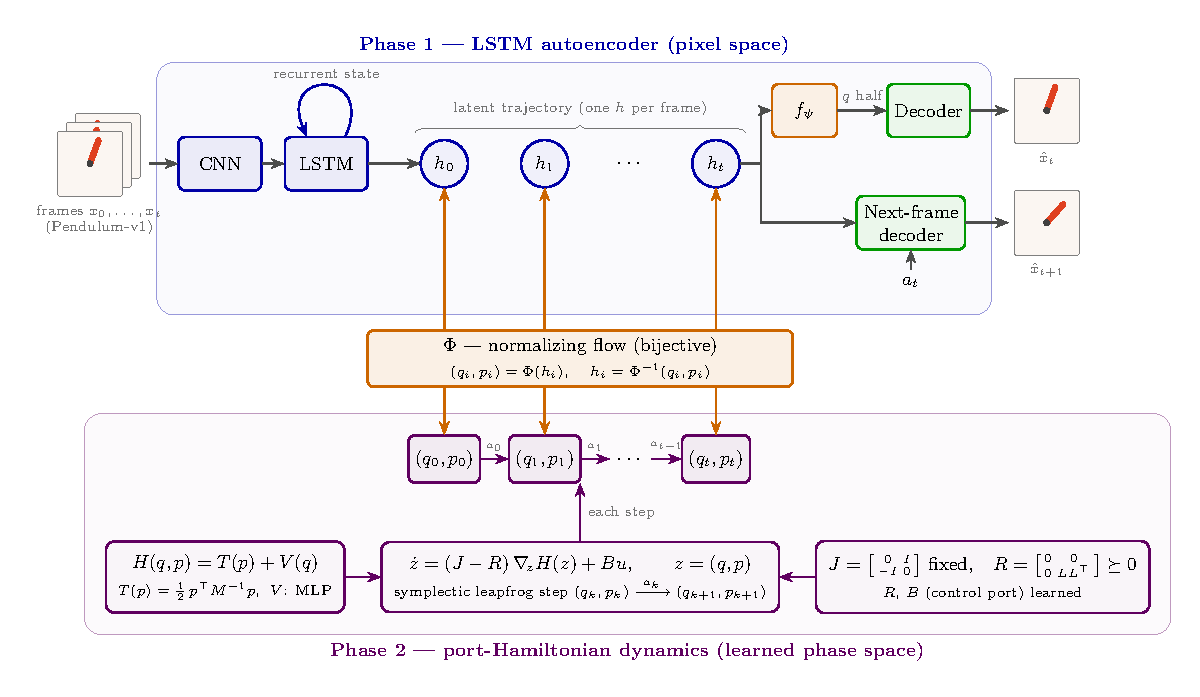
\includegraphics[width=\textwidth, height=0.95\textheight, keepaspectratio]{phamiltonian_arch.pdf}
  \end{center}
\end{frame}

%% ------------------------------------------------------------------
%% Slide 2 — linear probes on the latent trajectory
%% ------------------------------------------------------------------
\begin{frame}{Does $h_0, \dots, h_t$ encode angle and angular velocity?}
  Linear probe: least-squares fit $h_t \mapsto \bigl(\cos\theta,\ \sin\theta,\ \dot\theta\bigr)$,
  evaluated on held-out trajectories.

  \vspace{0.6em}
  \begin{center}
    \includegraphics[width=0.95\textwidth]{images/linearprobe.png}
  \end{center}

  \vspace{0.4em}
  $\Rightarrow$ the pendulum's phase space $(\theta, \dot\theta)$ is linearly decodable from $h$.
\end{frame}

\end{document}
